\documentclass{article}

%\usepackage[math,lf,footnotefigures]{MyriadPro}
\renewcommand\familydefault{\sfdefault} 
\usepackage[T1]{fontenc}

\usepackage{xparse}
\usepackage{tikz}
\usetikzlibrary{math}
\usetikzlibrary{arrows}
\usetikzlibrary{arrows.meta}
\usetikzlibrary{shapes.geometric}
\usetikzlibrary{shapes.misc}
\usetikzlibrary{positioning}
\usetikzlibrary{calc}

\tikzstyle{storage} = [rectangle, draw, line width=2pt, text centered, rounded corners, minimum height=2em, inner sep=8pt]
\tikzstyle{process} = [chamfered rectangle, draw, chamfered rectangle xsep=2cm, text centered, minimum height=2em, inner sep=6pt,fill=gray!20]
\tikzstyle{simplprocess} = [chamfered rectangle, draw, chamfered rectangle xsep=2cm, text centered, minimum height=2em, inner sep=6pt,fill=gray!40, dashed]
\tikzstyle{forcfunc} = [diamond, draw, aspect=2,inner sep=1pt]

\newcommand{\RiverDischarge}[3]{
	\begin{scope}[shift={#1},scale=#3]
		\coordinate (start) at (-3,1.25);
		\coordinate (xint1) at (-1,0);
		\coordinate (xint2) at (3,0);
		\coordinate (end) at (5,1.25);
		
		\coordinate (beg_11) at (2,-.5);
		\coordinate (beg_12) at ($(beg_11)-(1,0)$);		
		\coordinate (beg_21) at (0,-.5);
		\coordinate (beg_22) at ($(beg_21)+(1,0)$);
		\coordinate (center) at ($(beg_22)+(0,-.75)$);
		
		\coordinate (label) at ($(center)+(0,1.25)$);
		
		\fill[color=gray!80] 
		(xint1) parabola bend (center) ($(beg_22)+(0,.5)$);
		\fill[color=gray!80] 
		($(beg_22)+(0,.5)$) parabola bend (center) (xint2) ;
		
		\draw 
		(start) parabola (xint1)
		(xint1) parabola[bend at end] (center)
		(center) parabola (xint2)
		(xint2) parabola[bend at end] (end);
		
		\node[above,align=center] at (label) {#2};
	\end{scope}
}

\usepackage{color}

% define a new keyword
\makeatletter
\def\tikz@math@process@keyword@assign{%
	\tikz@math@collecttosemicolon{\tikz@math@process@keyword@@assign}%
}
\def\tikz@math@process@keyword@@assign{%
	\tikz@math@collected\tikz@math@parse
}
\makeatother


%% Let's reimplement TikZ arrays
\ExplSyntaxOn
\cs_new:Npn \shp #1 { \prop_show:c { l_tobias_array_#1_prop } }
\NewDocumentCommand{\definearray}{mO{}}
{% #1 = array name, #2 = items
	\prop_clear_new:c { l_tobias_array_#1_prop }
	\int_step_inline:nnnn { 0 } { 1 } { \clist_count:n { #2 } - 1 }
	{
		\prop_put:cnx { l_tobias_array_#1_prop } { ##1 } { \clist_item:nn { #2 } { ##1 + 1 } }
	}
}
\NewDocumentCommand{\setarrayitem}{mmm}
{% #1 = array name, #2 = index, #3 = value
	\prop_put:cff { l_tobias_array_#1_prop } { #2 } { #3 }
}
\NewExpandableDocumentCommand{\arrayitem}{mm}
{
	\prop_item:cf { l_tobias_array_#1_prop } { #2 }
}
\cs_generate_variant:Nn \prop_put:Nnn { cff }
\cs_generate_variant:Nn \prop_item:Nn { cf }
\ExplSyntaxOff


\usepackage[absolute,overlay]{textpos}  % to position textblocks at arbitary places - must be after color

% ----------------------------------------------
% width and height units for positioning textblocks
% ----------------------------------------------
\setlength{\TPHorizModule}{1cm} 
\setlength{\TPVertModule}{1cm}

\begin{document}
	
\pagestyle{empty}

\begin{textblock}{16.0}(0.0,12.0)
	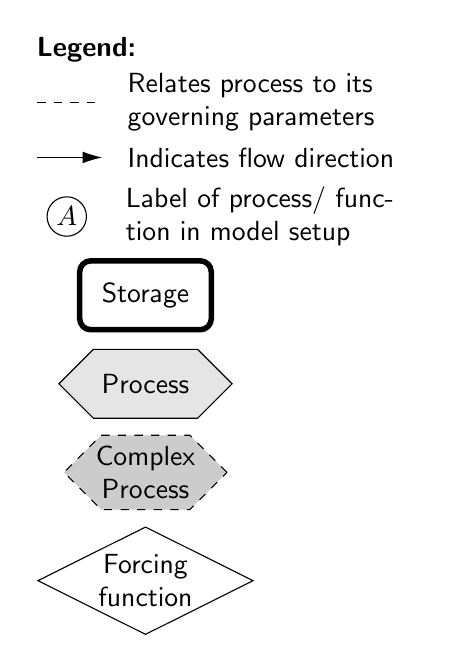
\begin{tikzpicture}[scale=2.5]				
		% legend caption
		\node[align=right] (A) at (0.0,0.0) {\textbf{Legend:}};
		% legend items
		\draw [dashed,text width=3.8cm] (-0.25,-0.27) -- (0.08,-0.27) node[right,xshift=0.2cm] {Relates process to its governing parameters};
		\draw [-{Latex[length=2.5mm, width=1.50mm]},text width=3.8cm] (-0.25,-0.55) -- (0.08,-0.55) node[right,xshift=0.2cm] {Indicates flow direction};
		\node [draw,circle,minimum size=0.5cm,inner sep=0pt] (circ) at (-0.1,-0.85) {\texttt{$A$}};
		\node [right of=circ,xshift=0.65cm,text width=3.8cm] at (0.3, -0.85) {Label of process/ function in model setup};
		\node [storage, align=center] at (0.3,-1.25) {Storage};
		\node [process, align=center] at (0.3,-1.70) {Process};
		\node [simplprocess, align=center,inner sep=1pt] at (0.3,-2.15) {Complex\\Process};
		\node [forcfunc, align=center] at (0.3,-2.7) {Forcing\\function};		
	\end{tikzpicture}
\end{textblock}


\begin{textblock}{16.0}(0.0,0.0)
	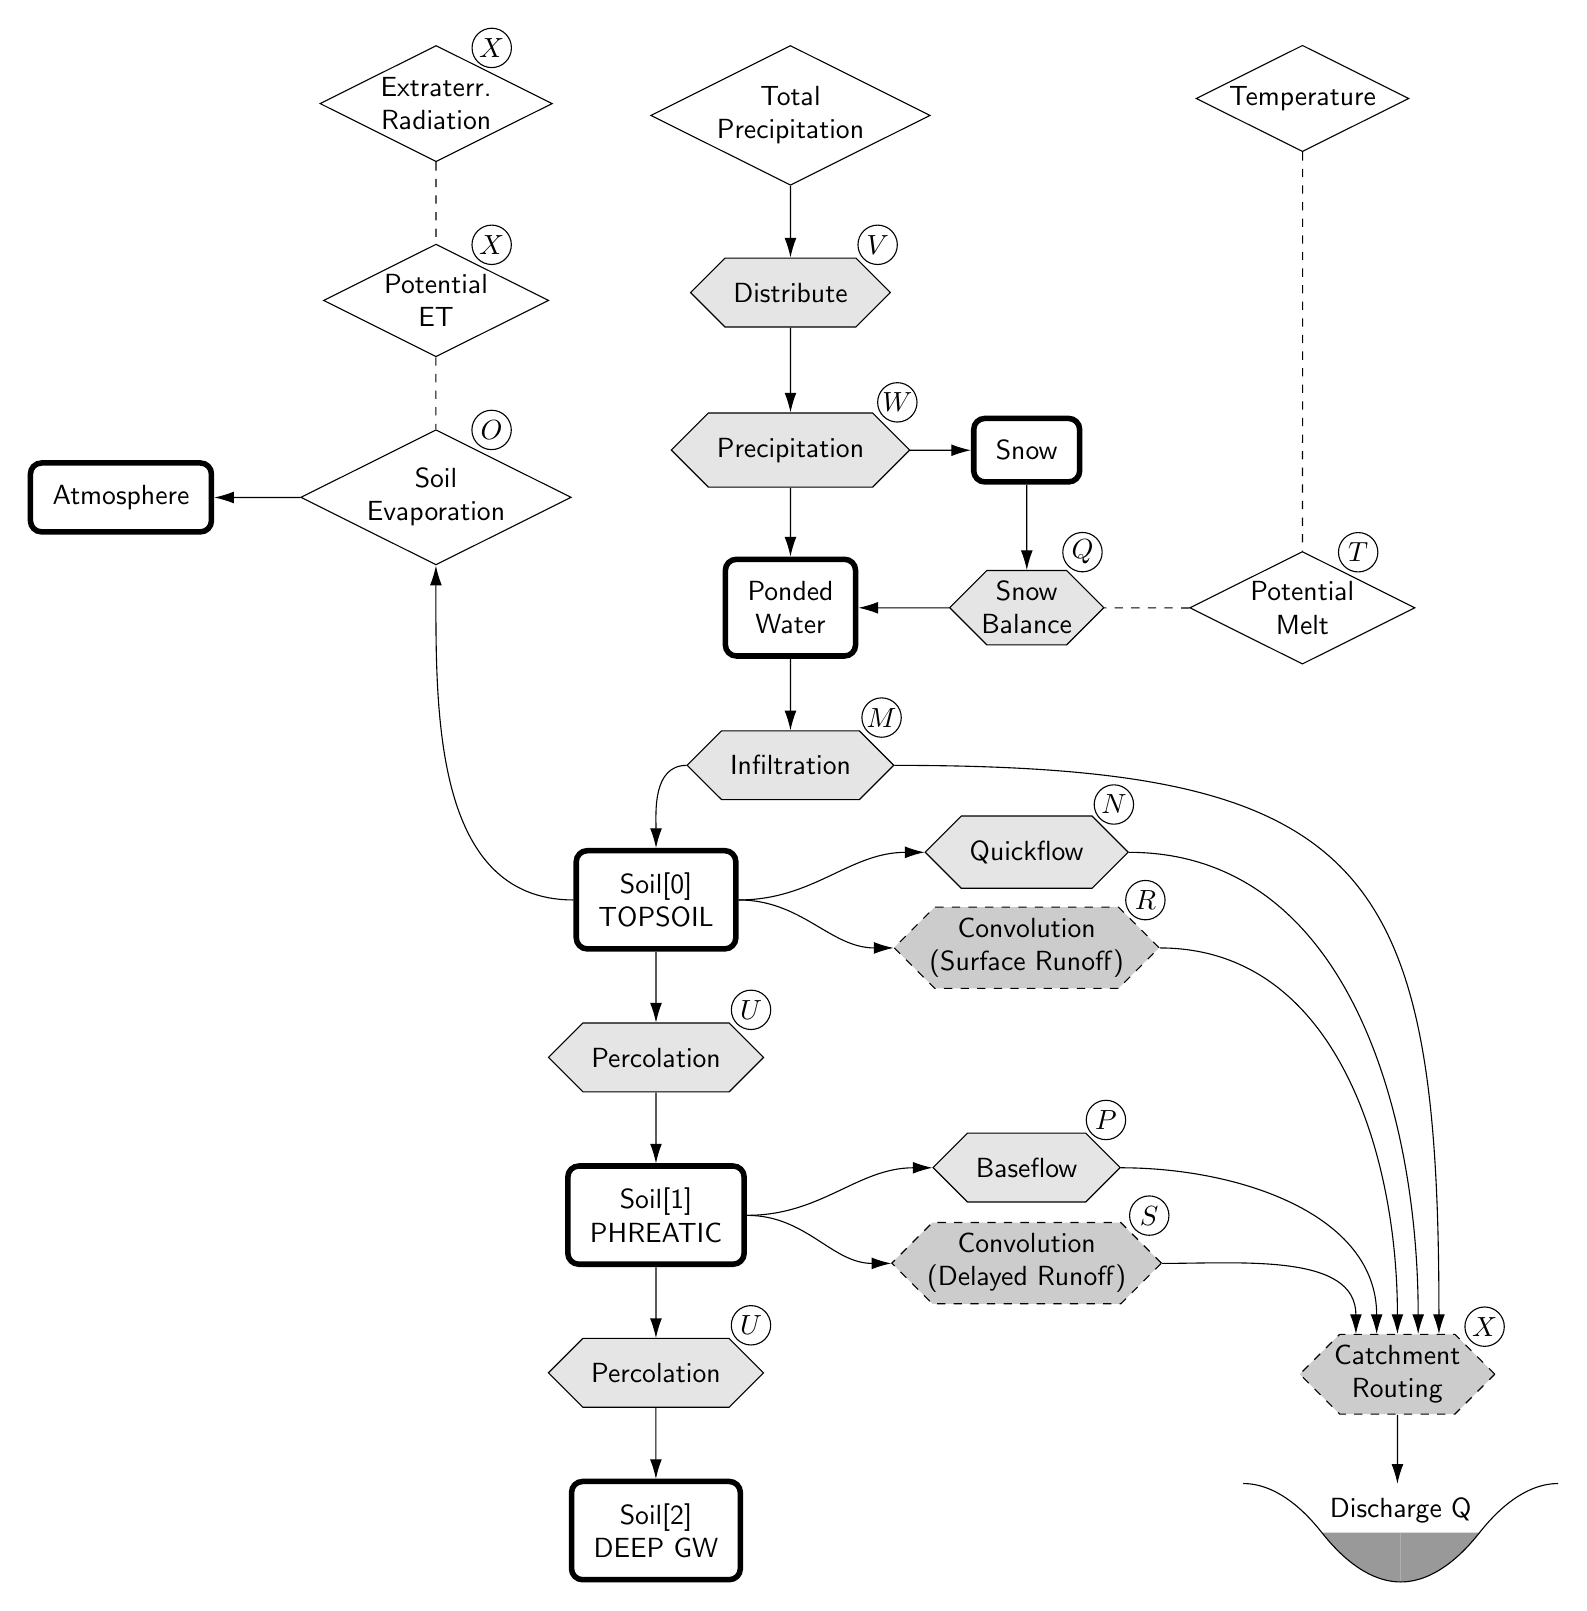
\begin{tikzpicture}[scale=2.5]

		\node [forcfunc, align=center] (A) at (0.0,0.0) {Total\\Precipitation};
		\node [process, align=center,below of=A,yshift=-1.25cm] (F) {Distribute};
		\node [process, align=center,below of=F,yshift=-1.0cm] (G) {Precipitation};
		\node [storage, align=center,right of=G,xshift=2.0cm] (I) {Snow};
		\node [process, align=center,below of=I,yshift=-1.0cm,inner sep=1pt] (J) {Snow\\Balance};
		\node [storage, align=center,below of=G,yshift=-1.0cm] (K) {Ponded\\Water};
		
		\node [forcfunc, align=center,left of=A,xshift=-3.5cm,yshift=0.15cm] (B) {Extraterr.\\Radiation};
		\node [forcfunc, align=center,below of=B,yshift=-1.5cm] (E) {Potential\\ET};
		\node [forcfunc, align=center,below of=E,yshift=-1.5cm] (H) {Soil\\Evaporation};
		\node [storage, align=center,left of=H,xshift=-3.0cm] (L) {Atmosphere};
		
		\node [forcfunc, align=center,right of=J,xshift=2.5cm] (D) {Potential\\Melt};
		\node [forcfunc, align=center,above of=D,yshift=5.47cm] (C) {Temperature};
		
		\node [process, align=center,below of=K,yshift=-1.0cm] (M) {Infiltration};
		\node [storage, align=center,below left of=M,xshift=-1cm,yshift=-1.0cm] (N) {Soil[0]\\TOPSOIL};
		\node [process, align=center,below of=N,yshift=-1.0cm] (O) {Percolation};
		\node [storage, align=center,below of=O,yshift=-1.0cm] (P) {Soil[1]\\PHREATIC};
		\node [process, align=center,below of=P,yshift=-1.0cm] (Q) {Percolation};
		\node [storage, align=center,below of=Q,yshift=-1.0cm] (R) {Soil[2]\\DEEP GW};
		
		\node [process, align=center,above right of= N,xshift=4.0cm,yshift=-0.1cm] (S) {Quickflow};
		\node [simplprocess, align=center,below right of=N,xshift=4.0cm,yshift=+0.1cm,inner sep=1pt] (T) {Convolution\\(Surface Runoff)};
		\node [process, align=center,above right of= P,xshift=4.0cm,yshift=-0.1cm] (U) {Baseflow};
		\node [simplprocess, align=center,below right of=P,xshift=4.0cm,yshift=+0.1cm,inner sep=1pt] (V) {Convolution\\(Delayed Runoff)};
		
		\node [simplprocess, align=center,below right of=V,xshift=4.0cm,yshift=-0.7cm,inner sep=1pt] (W) {Catchment\\Routing};
		
		% processes with multiple options
		\node[draw,above right of=M,xshift=0.45cm,yshift=-0.1cm,circle,minimum size=0.5cm,inner sep=0pt]  {\texttt{$M$}};
		\node[draw,above right of=S,xshift=0.4cm,yshift=-0.1cm,circle,minimum size=0.5cm,inner sep=0pt]  {\texttt{$N$}};
		\node[draw,above right of=H,yshift=0.15cm,circle,minimum size=0.5cm,inner sep=0pt]  {\texttt{$O$}};
		\node[draw,above right of=U,xshift=0.3cm,yshift=-0.1cm,circle,minimum size=0.5cm,inner sep=0pt]  {\texttt{$P$}};
		\node[draw,above right of=J,xshift=0.0cm,circle,minimum size=0.5cm,inner sep=0pt]  {\texttt{$Q$}};
		% processes with one option
		\node[draw,above right of=T,xshift=0.8cm,yshift=-0.1cm,circle,minimum size=0.5cm,inner sep=0pt]  {\texttt{$R$}};
		\node[draw,above right of=V,xshift=0.85cm,yshift=-0.1cm,circle,minimum size=0.5cm,inner sep=0pt]  {\texttt{$S$}};
		\node[draw,above right of=D,xshift=0.0cm,circle,minimum size=0.5cm,inner sep=0pt]  {\texttt{$T$}};
		\node[draw,above right of=O,xshift=0.5cm,yshift=-0.1cm,circle,minimum size=0.5cm,inner sep=0pt]  {\texttt{$U$}};
		\node[draw,above right of=Q,xshift=0.5cm,yshift=-0.1cm,circle,minimum size=0.5cm,inner sep=0pt]  {\texttt{$U$}};
		\node[draw,above right of=F,xshift=0.4cm,yshift=-0.1cm,circle,minimum size=0.5cm,inner sep=0pt]  {\texttt{$V$}};
		\node[draw,above right of=G,xshift=0.65cm,yshift=-0.1cm,circle,minimum size=0.5cm,inner sep=0pt]  {\texttt{$W$}};
		% processes without parameters
		\node[draw,above right of=B,xshift=0.0cm,circle,minimum size=0.5cm,inner sep=0pt]  {\texttt{$X$}};
		\node[draw,above right of=E,xshift=0.0cm,circle,minimum size=0.5cm,inner sep=0pt]  {\texttt{$X$}};
		\node[draw,above right of=W,xshift=0.4cm,yshift=-0.1cm,circle,minimum size=0.5cm,inner sep=0pt]  {\texttt{$X$}};
		
		% connections
		\draw[dashed] (B) -- (E);
		\draw[dashed] (E) -- (H);
		\draw[dashed] (C) -- (D);
		\draw[dashed] (D) -- (J);
		
		\draw[-{Latex[length=2.5mm, width=1.50mm]}] (A) -- (F);
		\draw[-{Latex[length=2.5mm, width=1.50mm]}] (F) -- (G);
		\draw[-{Latex[length=2.5mm, width=1.50mm]}] (G) -- (I);
		\draw[-{Latex[length=2.5mm, width=1.50mm]}] (I) -- (J);
		\draw[-{Latex[length=2.5mm, width=1.50mm]}] (J) -- (K);
		\draw[-{Latex[length=2.5mm, width=1.50mm]}] (G) -- (K);
		\draw[-{Latex[length=2.5mm, width=1.50mm]}] (K) -- (M);
		\draw[-{Latex[length=2.5mm, width=1.50mm]}] (H) -- (L);
		
		\draw[-{Latex[length=2.5mm, width=1.50mm]}] (M.west) to[out=180,in=90] (N.north);
		\draw[-{Latex[length=2.5mm, width=1.50mm]}] (N.west) to[out=180,in=270] (H.south);
		\draw[-{Latex[length=2.5mm, width=1.50mm]}] (N) -- (O);
		\draw[-{Latex[length=2.5mm, width=1.50mm]}] (O) -- (P);
		\draw[-{Latex[length=2.5mm, width=1.50mm]}] (P) -- (Q);
		\draw[-{Latex[length=2.5mm, width=1.50mm]}] (Q) -- (R);
		
		\draw[-{Latex[length=2.5mm, width=1.50mm]}] (N.east) to[out=0,in=180] (S.west);
		\draw[-{Latex[length=2.5mm, width=1.50mm]}] (N.east) to[out=0,in=180] (T.west);
		\draw[-{Latex[length=2.5mm, width=1.50mm]}] (P.east) to[out=0,in=180] (U.west);
		\draw[-{Latex[length=2.5mm, width=1.50mm]}] (P.east) to[out=0,in=180] (V.west);
		
		\draw[-{Latex[length=2.5mm, width=1.50mm]}] (M.east) to[out=0,in=90,distance=2.4cm] ([xshift=0.6em]W.north);
		\draw[-{Latex[length=2.5mm, width=1.50mm]}] (S.east) to[out=0,in=90] ([xshift=0.3em]W.north);
		\draw[-{Latex[length=2.5mm, width=1.50mm]}] (T.east) to[out=0,in=90] ([xshift=0.0em]W.north);
		\draw[-{Latex[length=2.5mm, width=1.50mm]}] (U.east) to[out=0,in=90] ([xshift=-0.3em]W.north);
		\draw[-{Latex[length=2.5mm, width=1.50mm]}] (V.east) to[out=0,in=90] ([xshift=-0.6em]W.north);
		
		% River Discharge
		\RiverDischarge{(2.9,-7.2)}{Discharge Q}{0.2}
		\draw[-{Latex[length=2.5mm, width=1.50mm]}] (W) -- ([yshift=-0.35cm]W.south);
				
	\end{tikzpicture}
\end{textblock}

\end{document}



